\section{Query User}
\placeholder{Summary of what query user does.}

\subsection{Parameters}
\begin{description}
    \item [firstName, lastName] The first and last name of the user to be queried.
\end{description}

\subsection{Results}
If the user exists, the column of the user will be returned. If the user does not exist, not such column will be returned.

\begin{center}
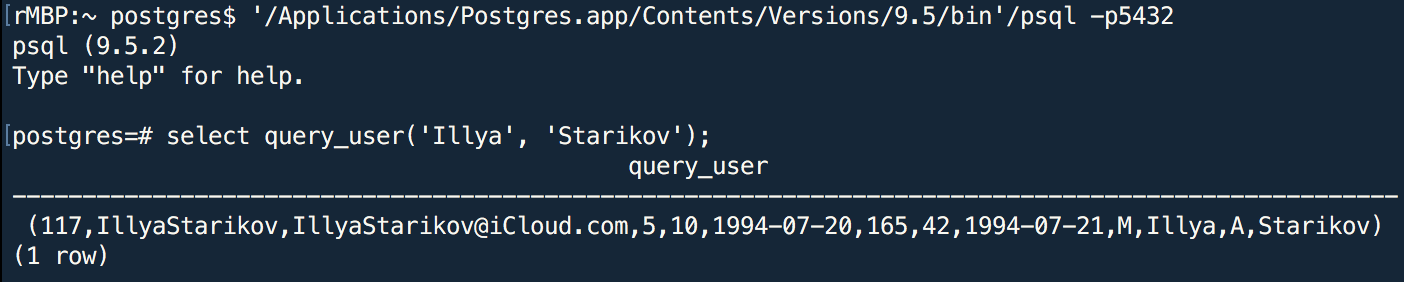
\includegraphics[width=\columnwidth]{include/assets/screenshots/query_user}
\end{center}